⁵\documentclass[norsk]{article}
\usepackage[utf8]{inputenc}
\usepackage{graphicx}
\usepackage{enumitem}
\usepackage{float}
\usepackage{refcount}
\usepackage{calc}

%Sets the languages
\usepackage[norsk, english]{babel}

%Configuration of numbered list
\newlist{legal}{enumerate}{10}
\setlist[legal]{label*=\arabic*.}


\title{Prosjektdokumentasjon i Software Engineering og Testing 2019}
\author{Jonas Braut \\ Sivert Skarning \\ Nikolai Svanåsbakken \\Oscar L. Ramstad \\ Amalie Y. Ressler}
\date{Oktober 2019}

\begin{document}

\maketitle
\newpage
\tableofcontents
\newpage
\section{Presentasjon av oppgaven}

\subsection{Introduksjon} 

Formålet med denne oppgaven er å lage/definere et system som omhandler infrastrukturen rundt sportsarrangement, og deres dannelse/registrering/osv., i tråd med økende antall mennesker som deltar eller ønsker å delta i sportsarrangementer.\\
Dette systemet vil være et felles system som vil bli tatt i bruk av mindre klubber eller sportsstiftelser, ettersom disse organisasjonene gjerne ikke har kapasitet til ha en egen infrastruktur rundt det å holde arrangementer eller å reklamere disse arrangementene. 

\section{Systembeskrivelse}
Dette er et system som skal fungere som et slags knutepunkt for mindre klubber, sportsstiftelser og utøvere. Via dette systemet skal disse klubbene være i stand til å registrere sine utøvere til arrangementer, i tillegg til å kunne arrangere sine egne arrangement. Utøvere skal kunne få innformasjon om kommende arrangementet, ha mulighet til påmelding og holde seg oppdatert helt fram til arrangementet er avsluttet. Systemet skal ikke være et sosialt medium, og dermed skal ikke "forbindelser", kommentering, eller andre lignende sosiale funksjoner være med.

\subsection{Brukere}
\begin{enumerate}
    \item Administrator\\
    En administrator har, i bunn og grunn, mulighet til å gjøre hva som helst når det kommer til å administrere arrangementer og klubber/klubbmedlemmer. En administrator skal kunne se alle klubber og arrangementer registrert i systemet, samt potensielt redigere/slette disse.\\
    En administrator vil først og fremst være en supportbruker, ment for å hjelpe klubber som har problemer med navigering/registrering i systemet.
    \item Klubb\\
    En klubbruker er en representant av klubben i systemet. Brukeren tar hånd om registrering av utøvere, inndeling i lag/aldersgrupper og opprettelse av arrangement. Brukeren kan kun se sin egen klubb og dens medlemmer.
    \item Nettbruker\\
    En nettbruker er ikke en registrerbar brukertype, og referer til alle som tar i bruk av nettsiden. Det vil si at de kan kun ta i bruk nettsiden, uten noen persistent lagring av deres data. Ved bruk av nettsiden skal nettbrukere være i stand til å finne arrangementer og relatert informasjon, søke opp utøvere og deres resultater,
\end{enumerate}

\subsection{Applikasjon}
Dette er en applikasjon som skal tas til bruk på et nettbrett eller smart telefon. Applikasjonen skal ha en login-skjerm. På denne skjermen skal man kunne skrive inn brukernavn og passord, samt kunne kontakte support i det tilfellet man har glemt brukernavn og/eller passord. Applikasjonen skal kunne la brukeren håndtere mest mulig av det som angår deltagere på et arrangement, fra å kunne opprette arrangementet til å kunne fylle ut resultatlister etter avsluttet arrangement. 

\subsection{API}
API-et er en kritisk del av systemet som skal kommunisere med ubegrenset antall brukere. Den vil bli brukt til å overføre data på en strukturert måte, mellom websiden, applikasjon og databasen. API-et skal ta i mot forespørsler fra webside og applikasjon om blant annet liste av arrangementer, terminlister, utøverdata, login i applikasjon og registrere medlemmer/arrangementer.\\ \\
Tilstandsdiagram - \textit{Figure \ref{fig:state-api-get}} viser eksempel på syklusen til et GET kall til API-et. API-et vil motta forespørsler fra kilent (webside/applikasjon) og vil deretter sende SQL-spørring til databasen hvis forespørselen er gyldig. API-et svarer til klienten med data fra databasen eller feilmelding hvis noe gikk galt. \\ \\
\textit{Figure \ref{fig:get-at-api}} viser eksempel på et API kall fra applikasjon for å hente ut utøvere fra databasen.\\ \\
\textit{Figure \ref{fig:post-at-api}} viser eksempel på et API kall fra applikasjon for å legge til en utøver i databasen.\\

\begin{figure}[H]
\centering 
    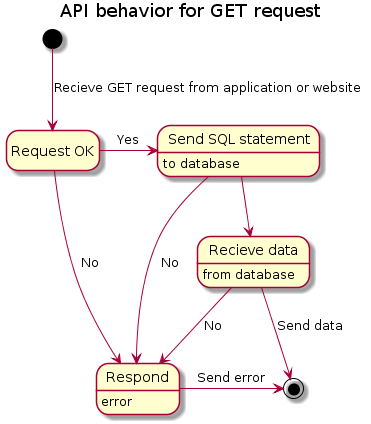
\includegraphics[scale=0.7]{images/state-api-get.png}
    \caption{API GET kall fra en klient for henting av data fra databasen.}\label{fig:state-api-get}
\end{figure}
\begin{figure}[H]
\centering 
    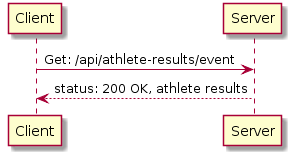
\includegraphics[scale=0.7]{images/get-athletes-api-call.png}
    \caption{GET kall for henting av utøvere}\label{fig:get-at-api}
\end{figure}
\begin{figure}[H]
\centering 
    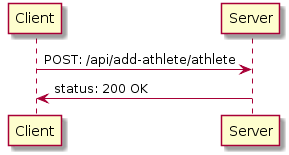
\includegraphics[scale=0.7]{images/post-athletes-api-call.png}
    \caption{POST kall for opplasting av utøvere}\label{fig:post-at-api}
\end{figure}

\subsection{Nettside}
Dette er en nettside som kun skal inneholde aggregert data fra arrangementer og klubber. Det skal være en kalenderfunksjon på nettsiden, som skal inneholde all relevant data rundt et arrangement (tid, sted, arrangør o.l.). Nettsiden skal inneholde en enkel søkemotor for å potensielt forenkle navigasjon gjennom nettsiden. Det skal være egne sider for registrerte klubber, med korte introduksjoner av klubbene samt kontaktinformasjon.\\
Nettsiden skal inneholde lister av registrerte klubber, registrerte utøvere, lag- og aldersgruppeoppdeling, og disse listene skal kunne sorteres (både stigende og senkende) alfabetisk, på klubb alfabetisk, område alfabetisk, lag/aldersgruppe alfabetisk. Det skal også være lister over arrangementer og resultater, og disse skal kunne sorteres via relevant informasjon (navn, sted, tid osv.).\\
Forsiden skal inneholde kortfattet informasjon om aktuelle arrangementer som enten foregår for øyeblikket, eller som starter i løpet av en vilkårlig tidsperiode.
%Nice%

\subsection{Database}
Databasen skal lagre all informasjon som blir sendt fra applikasjon til databasen blant annet når arrangement legges til, redigeres, fjernes; når utøvere legges til, redigeres, fjernes; når klubber legges til, redigeres, fjernes, og alle andre relevante data fra applikasjonen. Dette skjer via kall til API, så selve applikasjonen kan ikke direkte forandre på databasen.\\
Mer informasjon om dataene og database strukturen finnes under \textit{Database} senere i dokumentet.

\section{Krav}
Systemets kravspesifikasjon inneholder de teknisk funksjonelle og ikke-funksjonelle kravene til systemet, og hvordan systemet fungerer i sin helhet.

    % UNDER HER ENDRER VI LISTEFORMEN TIL FUNKSJONALITET I STEDET FOR LOKASJON %
\subsection{Funksjonelle krav}
\begin{legal}
    \item Søking
    \begin{legal}
        \item Alle skal kunne søke etter arrangementer, nettside.
        \item Alle skal kunne søke etter terminlister, nettside.
        \item Alle skal kunne søke i terminlister, nettside.
        \item Alle skal kunne søke etter klubber, nettside.
        \item Alle skal kunne søke etter utøveres profil, nettside.
    \end{legal}
    \item Registrering
    \begin{legal}
        \item Klubb-brukere registreres via å sende en mail til driftsansvarlig.
        \item Klubb skal kunne legge til kommende arrangementer ved å trykke på et valg i dropdown-menyen.
        \begin{legal}
            \item Klubber kan kun slette egne arrangementer.
        \end{legal}
        \item Klubb skal kunne legge inn utøverdata.
        \item Klubb skal kunne opprette konkurranser for kommende arrangementer.
        \item Arrangerende klubb skal kunne melde opp utøvere til en opprettet konkurranse. 
        \item Klubb skal kunne registrere medlemmer.
        \begin{legal}
            \item En klubb skal kunne dele inn medlemmer i lag/aldersgrupper.
            \item En klubb skal kunne redigere medlemmer.
        \end{legal}
    \end{legal}
    \item Kalender
    \begin{legal}
        \item Alle skal kunne se kalender for inneværende måned med arrangementer og trykke seg tilbake til forrige måned eller frem til neste måned, nettside.
        \item Alle skal kunne laste ned kalenderdata, nettside.
        \item Alle skal kunne se kalenderdata på websiden, nettside.
        \item Alle skal kunne spesifisere ønsket sport som vises i kalender, nettside.
        \item Bruker skal kunne laste ned kalender data, nettside.
        %Husk, legg til krav om kaleneder for Applikasjon%
    \end{legal}
    \item Resultatliste, applikasjon
    \begin{legal}
        \item Klubb skal kunne registrere utøvers resultater i form av en resultatliste.
        \item Under opprettelse av liste skal klubb kunne velge en opprettet konkurranse.
        \item Under opprettelse av liste skal klubb kunne legge til tid og etter-tid (tiden alle andre har kommet inn etter førsteplassen) for hver deltager.
        \item Resultatlisten skal sendes til API et. 
    \end{legal}
    \item Resultatliste, nettside 
    \begin{legal}
        \item Alle skal kunne velge hvilket arrangement de ønsker å se resultatlistene til. 
        \item Alle skal kunne velge hvilken konkurranse de ønsker å se resultatlistene til.
        \item Alle skal kunne velge kjønn. 
        \item Alle skal kunne velge fra dato. 
        \item Alle skal kunne velge til dato.
        \item Alle skal kunne søke på bakgrunn av fødselsår. 
    \end{legal}
    \item Diverse jeg ikke vet hvor jeg skal putte
    \begin{legal}
        \item En klubb skal ikke kunne se en annen klubb utover arrangement-/kalenderdata.
        \item En klubb skal kunne vise utøverdata.
        \item Alle skal kunne se detaljer om arrangementer, nettside.
        \item Etter innlogging skal en meny med knapper vises for klubb og admin.
        \item Systemet skal kunne ta i mot data og importere det til API, database.
        \item Systemet skal bare gi lese rettigheter til webside, API.
    \end{legal}

    \subsection{Ikke-funksjonelle krav}
    \item Applikasjon
    \begin{legal}
        \item Applikasjonen skal følge lov og forskrifter for universell. utforming.
        \item Kalenderdata skal kunne bli synkronisert med Google Calendar-API
        \item Klubb og Admin skal kunne få hjelp ved glemt passord innen 15 min etter gjennomført glemt-passord prosess. 
        \item GUI skal være enkelt å bruke. %ikke målbart%
        \begin{legal}
            \item Brukeropplæring skal dermed ikke ta mer enn 10 min. 
            \item Det skal ikke komme mer enn 2 spørsmål, til support, i måneden relatert til bruk
        \end{legal}
    \end{legal}
    \item Nettside 
    \begin{legal}
        \item Nettsiden skal følge lov og forskrifter for universell utforming.
    \end{legal}
    \item Database
    \begin{legal}
        \item Databasen skal kjøre MySQL
        \item Databasen skal leve i Amazon sin skytjeneste.
    \end{legal}

\subsection{Krav til brukergrensesnitt}
% replace this list with mockup GUI image%
    \item Applikasjon, gjeldene alle vinduer 
    \begin{legal}
        \item Applikasjonen skal kunne skalere etter brukeren sin enhetsstørrelse.
        \item Logo til applikasjon skal vises på siden.
    \end{legal}
    \item Applikasjon, innloggingsside
    \begin{legal}
        \item Klubb og Admin skal kunne skrive inn brukernavn.
        \item Klubb og Admin skal kunne skrive inn passord.
        \item Klubb og Admin skal kunne logge inn med en knapp.
        \item Klubb skal kunne få hjelp om de har glemt passord.
        \item Klubb skal kunne trykke på en glemt-pasord knapp for å starte prosessen.
    \end{legal}
    \item Applikasjon, forside, meny
    \begin{legal}
        \item Etter innlogging skal en meny med knapper vises for klubb og admin.
        \item Menyen skal gi tilgang til opprettelse av arrangementer.
        \item Menyen skal gi tilgang til opprettelse av konkurranser.
        \item Menyen skal gi tilgang til en kalender.
    \end{legal}
\end{legal}

\section{Prosjektets arbeidsomfang}
Prosjektets krav er blitt estimert for å bedre kunne prioritere og delegere arbeidsoppgaver. Nedenfor finner du tabeller sortert etter krav, med tilhørende tidsestimat og prioritet.\newline
Tidsestimat og prioritet er gitt ved t-skjorte størrelser. Dette gjør det lettere for teamet å kunne sortere arbeidsoppgaver etter omfang uten at man føler seg bundet av at en oppgave skal ta et spesifikt anatall timer eller dager. Estimering av antall timer er umulig og det blir derfor nyttigere å angi arbeidsomfang med t-skorte størrelser. Størrelsene er small, medium og large.

\begin{table}[ht]
\begin{tabular}{|l|l|l|l|}
\hline
%Må gå over disse på nytt%
Krav & Tidsestimat & Forretningsnytte & Prioritet           \\ \hline
1.1-1.5 Webside søkemotor            & S    & S     &       \\ \hline
1.5-1.9 Webside søkemotor            & S    & S     &       \\ \hline
1.10    Webside utøverdata           & S    & S     &       \\ \hline
1.11    Webside arrangement detaljer & M    & M     &       \\ \hline
2.1     Applikasjon innlogging       & S    & L     &       \\
\hline
2.2  & S           & S      &       \\ \hline
2.3  & L           & L      &       \\ \hline
2.5  & M           & S      &       \\ \hline
2.6  & S           & M      &       \\ \hline
2.7  & S           & M      &       \\ \hline
2.8  & S           & L      &       \\ \hline
2.9  & S           & M      &       \\ \hline
2.10 & S           & L      &       \\ \hline

\end{tabular}
\end{table}

\section{Use Case} % Del opp use cases i sealevel / fishlevel hvis vi får nok use cases. %
    \subsection{Klubb legger til et arrangement} 
    \begin{figure}[H]
    \centering
        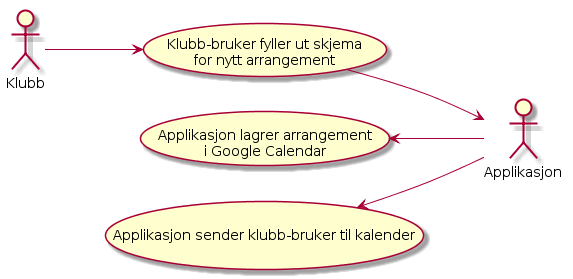
\includegraphics[scale=0.7]{images/uc-klubb-legger-til-arrangement.png}
        \caption{Use Case: Klubb legger til et arrangement.}\label{fig:uc-add-event}
    \end{figure}
    \textbf{Aktør:} Bruker, Applikasjon, API, Database.\newline
        \textbf{Trigger:} Bruker trykker på knapp for å opprette arrangementer i kalenderen, på applikasjonen.\newline
        \textbf{Pre-betingelse:} Brukeren må ha en klubb-brukerkonto i systemet. Enheten applikasjonen kjører på må ha tilgang til internett.\newline
        \textbf{Post-betingelse:} \newline
        Minimal suksess: Arrangementet blir opprettet i kalenderen.\newline
        Maksimal suksess: Arrangementet blir opprettet i kalenderen og brukeren blir sendt videre til kalenderen, hvor det nye arrangementet er synlig. \newline

        \textbf{Normal hendelsesflyt:}
        \begin{enumerate}
            \item Klubb-bruker logger inn i applikasjon.
            \item Klubb-bruker navigerer seg frem til kalender.
            \item Klubb-bruker trykker på knapp for oppretting av arrangement.
            \item \label{itm:1A} Klubb-bruker fyller ut skjema for nytt arrangement.
            \item \label{itm:1B} Applikasjonen  sender forespørsel til API for å lagre kalenderdata.
            \item API sender SQL-spørring til databasen for å lagre kalenderdata.
            \item \label{itm:1C} Databasen kjører SQL-spørring og responderer med HTTP-protokoll kode 200 (OK).
            \item API gir respons til applikasjon.
            \item Applikasjon går tilbake til kalender(eller arrangementer?) siden, hvor det nye arrangementet er synlig.
            \newline
        \end{enumerate}
        
        \textbf{Variasjoner i hendelsesflyt:}
        
        \begin{enumerate}[start={\getrefnumber{itm:1A}}]
            \item Bruker fyller inn ugyldig informasjon i skjema.
                \begin{enumerate}
                    \item Applikasjon viser hvilke felter som er feil.
                \end{enumerate}
            \setcounter{enumi}{\getrefnumber{itm:1B}{-1}}
            \item Applikasjon har ikke tilgang til internett.
                \begin{enumerate}
                    \item Applikasjonen lagrer data midlertidig.
                    \item Applikasjonen viser en feilmelding til bruker om å koble til internett.
                \end{enumerate}
            \setcounter{enumi}{\getrefnumber{itm:1C}{-1}}
            \item Databasen hindres i å lagre kalenderdata.
                \begin{enumerate}
                    \item Databasen responderer til API med feilkode.
                    \item Applikasjon får respons fra API og viser bruker feilkode.
                    \item Applikasjon ber bruker å prøve på nytt.
                \end{enumerate}
        \end{enumerate}

    \subsection{Klubb legger til resultater}
    \begin{figure}[H]
        \centering
            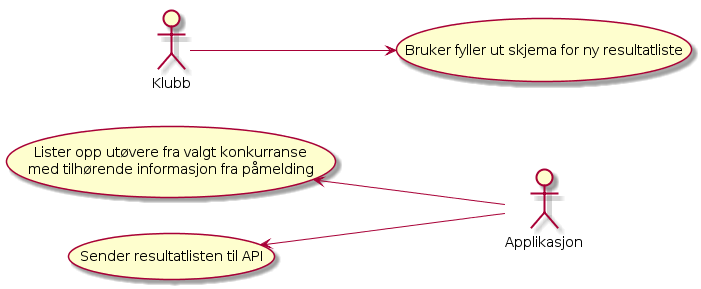
\includegraphics[scale=0.55]{images/uc-add-athlete-results.png}
            \caption{Use Case: Klubb legger til en resultatliste.}\label{fig:uc-add-athlete-results}
        \end{figure}
    \textbf{Aktør:} Bruker, Applikasjon, API, Database.\newline
    \textbf{Trigger:} Bruker trykker på knapp for å opprette resultatliste i applikasjonen. \newline
    \textbf{Pre-betingelse:} Bruker må ha klubb-brukerkonto i systemet. 
    Den gjeldende konkurransen må være opprettet.
    Den gjeldende konkurransen må være fullført og avsluttet.\newline
    \textbf{Post-betingelser:} Minimal og maksimal suksess: Resultatlisten blir opprettet og tilgjengelig for alle typer brukere. \newline

    \textbf{Normal hendelsesflyt:}
    \begin{enumerate}
        \item Klubb-bruker logger inn i applikasjon. 
        \item \label{itm:2A}Klubb-bruker trykker på knapp for oppretting av resultatliste.
        \item Klubb-bruker velger gjeldende konkurranse. 
        \item \label{itm:2B}Applikasjon lister opp utøvere fra valgt konkurranse med tilhørende informasjon fra påmelding.
        \item Klubb fyller ut resterende informasjon (tid, etter) 
        \item Applikasjonen sender forespørselg til API for å lagre resultatlisten. 
        \item \label{itm:2C}API sender SQL-spørring til databasen for å lagre resultatlisten. 
        \item Databasen kjører SQL-spørring og responderer med HTTP-protokoll kode 200(OK).
        \item API gir respons til applikasjonen. 
        \item Applikasjonen går tilbake til skjema siden for opprettelse av resultatliste. 
    \end{enumerate}
    
    \textbf{Variasjoner i hendelsesflyt:}
        \begin{enumerate}[start={\getrefnumber{itm:2A}}]
            \item Bruker fyller inn ugyldig informasjon i skjema.
                \begin{enumerate}
                    \item Applikasjon viser hvilke felter som er feil.
                \end{enumerate}
            \setcounter{enumi}{\getrefnumber{itm:2B}{-1}}
            \item Applikasjon har ikke tilgang til internett.
                \begin{enumerate}
                    \item Applikasjonen viser en feilmelding til bruker om å koble til internett.
                    \item Applikasjon har ikke tilgang til konkurranser. 
                    \item Applikasjon har ikke tilgang til utøverdata fra påmelding. 
                \end{enumerate}
            \setcounter{enumi}{\getrefnumber{itm:2C}{-1}}
            \item Databasen hindres i å lagre resultatdata.
                \begin{enumerate}
                    \item Databasen responderer til API med feilkode.
                    \item Applikasjon får respons fra API og viser bruker feilkode.
                    \item Applikasjon ber bruker å prøve på nytt.
                \end{enumerate}
        \end{enumerate}
        
\section{Sekvensdiagram}
\subsection{Registrere utøvers resultater}

\textbf{Hensikt:} Sekvensdiagrammet "Registrer resultater" gir en dypere forståelse av \textit{Use case 5.2} og illustrerer kommunikasjonen mellom applikasjonen og de andre komponentene i systemet. Denne kommunikasjonen oppstår når en klubb forsøker å opprette en resultatliste. 
\begin{figure}[H]
\centering 
    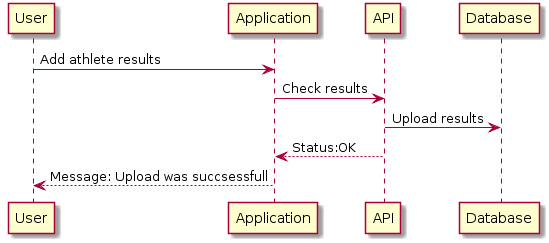
\includegraphics[scale=0.55]{images/add-athlete-results}
    \caption{Sekvensdiagram for å registrere utøvers resultater}\label{fig:add-at-res}
\end{figure}

\subsection{Populere resultater fra arrangement på nettsted}

\textbf{Hensikt:} Sekvensdiagrammet "Populer resultater" tar for seg den tekniske kommunikasjonen mellom nettsiden og andre komponenter som, applikasjon, API og database. Denne kommunikasjonen oppstår når en bruker ønsker å få se resultater til en konkurranse.
%Endre navngiving i sekvens diagrammet for å være konsistent, om ikke meningen var å vise alle resultatlistene til et arrangement. %
\begin{figure}[H]
\centering 
    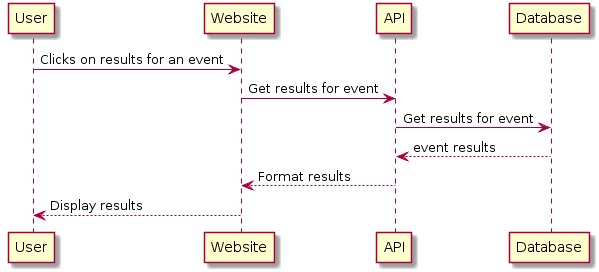
\includegraphics[scale=0.5]{images/get-athletes}
    \caption{Sekvensdiagram for henting av resultater fra arrangement}\label{fig:get-at-res}
\end{figure}


\subsection{Registrer et lag}
\textbf{Hensikt:} Sekvensdiagrammet "Registrer lag" tar for seg den tekniske kommunikasjonen mellom applikasjon og de andre komponentene som API og database. Denne kommunikasjonen oppstår når en klubb ønsker å registrere et tilhørende lag bestående av utøvere. 
\begin{figure}[H]
\centering
    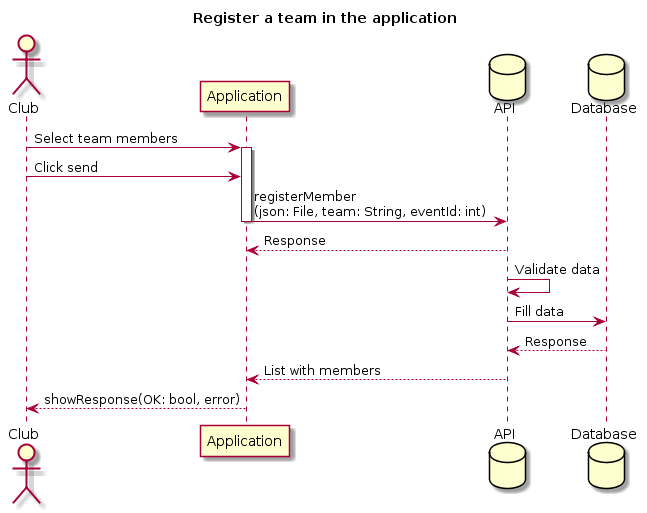
\includegraphics[scale=0.5]{images/register-team.png}
    \caption{Sekvensdiagram for registrering av et lag i applikasjonen.}\label{fig:register-team}
\end{figure}

\section{Arkitektur}
\subsection{Lagdeling}
\subsubsection{Moduler}
Lagdeling i kode er viktig, spesielt på systemer med et visst omfang. Løst koplet kode gjøre at enheter av koden lett kan bli byttet ut med andre implementasjoner hvis noe skal endres. Dette gjøre at kodebasen blir mer modulær og mer vedlikeholdbart.
I dette prosjektet er det gjort en rekke valg for å gjøre koden mer løst koplet.
Prototypen består av to moduler, Client og Models. Client sin oppgave er å håndtere interaksjon med bruker via GUI laget i JavaFX og "kontrollere" som håndterer data til GUI.
Models inneholder modellene som har implementasjonen av de egendefinerte datatypene og business logikk.
Det at disse to er to forskjellige moduler gjør at man lettere kan bytte de ut ved behov. Business logikken lever kanskje lenge, og endres kanskje ikke så mye som clienten som må holdes oppdatert etter hvilke enheter brukeren benytter.

\subsubsection{Repository pattern}
I prototypen har vi brukt repository pattern for å abstrahere datalaget i applikasjonen. Man lager et repository for alle modellene. Repository inneholder funksjoner slik som add og delete slik at man henter objektet man trenger i repositoriet og legger det tilbake etter man er ferdig med det.
Funksjonaliteten med hvordan data blir lagret er dermed gjemt for programmereren. Repositoriet kan følgelig byttes ut ved bytte av datalag.

\subsection{Database}
Prosjektet bruker en EER-modell for å fremstille databasen til systemet. Entitetstypene(tabellene) er delt inn på best mulig måte for å unngå gjentagende data. I tillegg vil all informasjon som ønskes av systemet finnes som attributter/kolonner, eller kan beregnes ut fra disse.
%Endre navngiving for å holde modellen konsistent%
    \begin{figure}[H]
    \centering 
        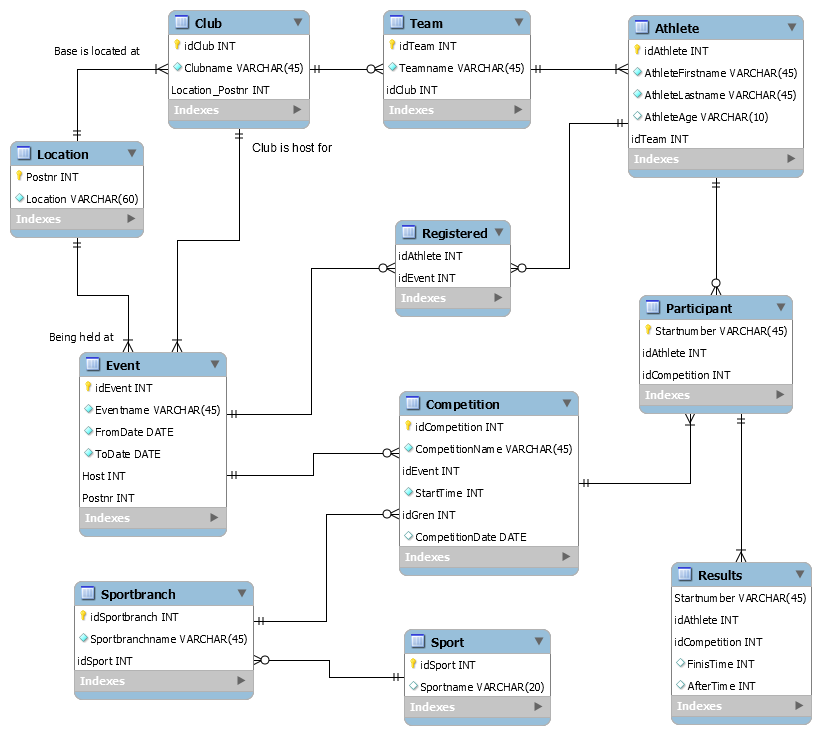
\includegraphics[scale=0.5]{images/datamodel.png}
        \caption{EER-model for å fremstille databasen til systemet}\label{fig:datamodel}
    \end{figure}
\section{Testing}
\section{Prototype}
Klubb- og adminknappene i det første vinduet er kun ment som en abstraksjon av innloggingsprosessen.

\section{Klasse-diagram}
\begin{figure}[H]
\centering
    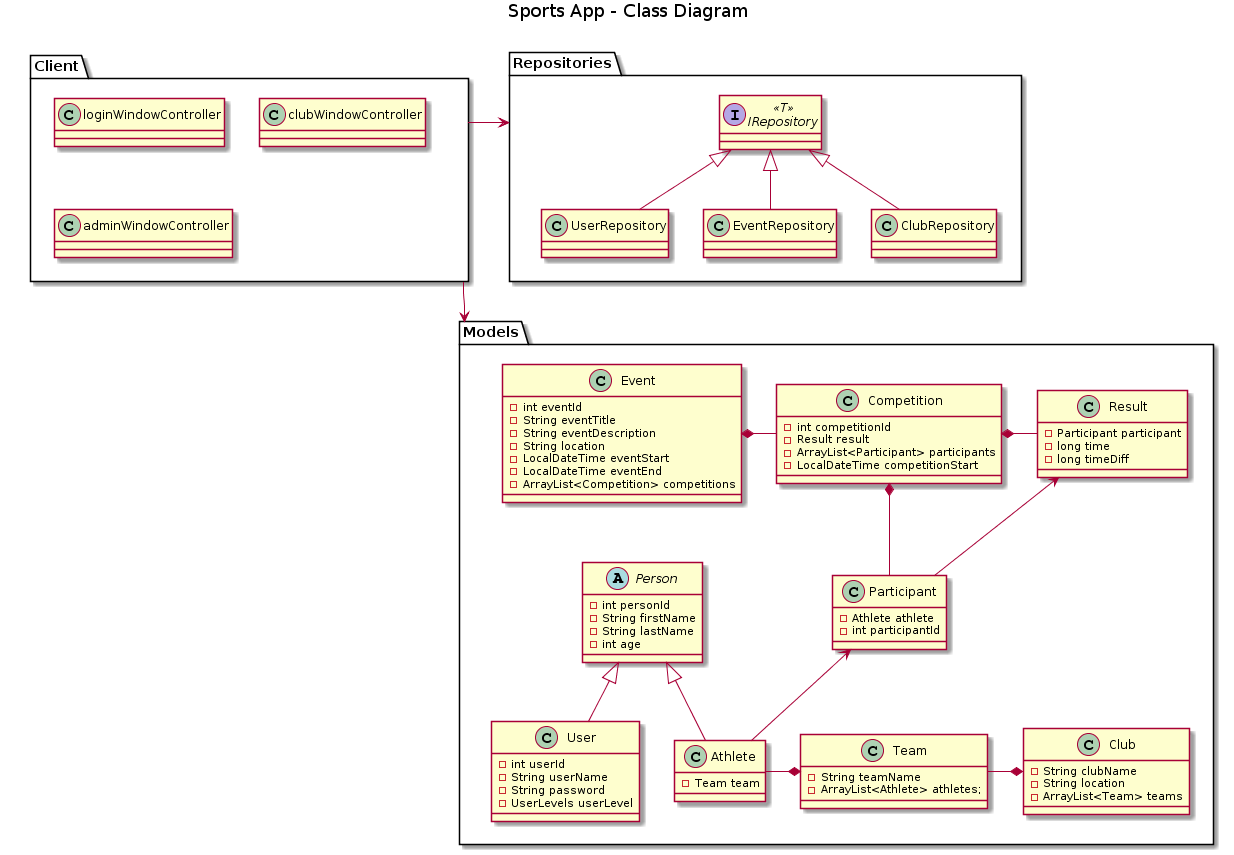
\includegraphics[scale=0.3]{images/class-uml.png}
    \caption{Klasse-diagram}\label{fig:class-uml}
\end{figure}
\end{document}
